
\documentclass{beamer}

\usepackage{hyperref}
\usetheme{Singapore}
\usecolortheme[RGB={0, 32, 91}]{structure}  % Rice blue
\setbeamertemplate{navigation symbols}{\insertframenumber}

\definecolor{riceblue}{rgb}{0.000, 0.125, 0.357}
\definecolor{ricegray}{rgb}{0.486, 0.494, 0.498}
\definecolor{ricerichblue}{rgb}{0.039, 0.314, 0.620}

\title{Pitch trajectory density estimation \\ for predicting future outcomes}
\author{\color{ricerichblue} Scott Powers and Vicente Iglesias}
\date{Saberseminar 2023}

\begin{document}

  \begin{frame}
    \maketitle
    \vfill
    \hfill
    
\includegraphics[width = 0.5\textwidth]{images/rice_smgt.png}
  \end{frame}

  \begin{frame}{Pitch Modeling}
    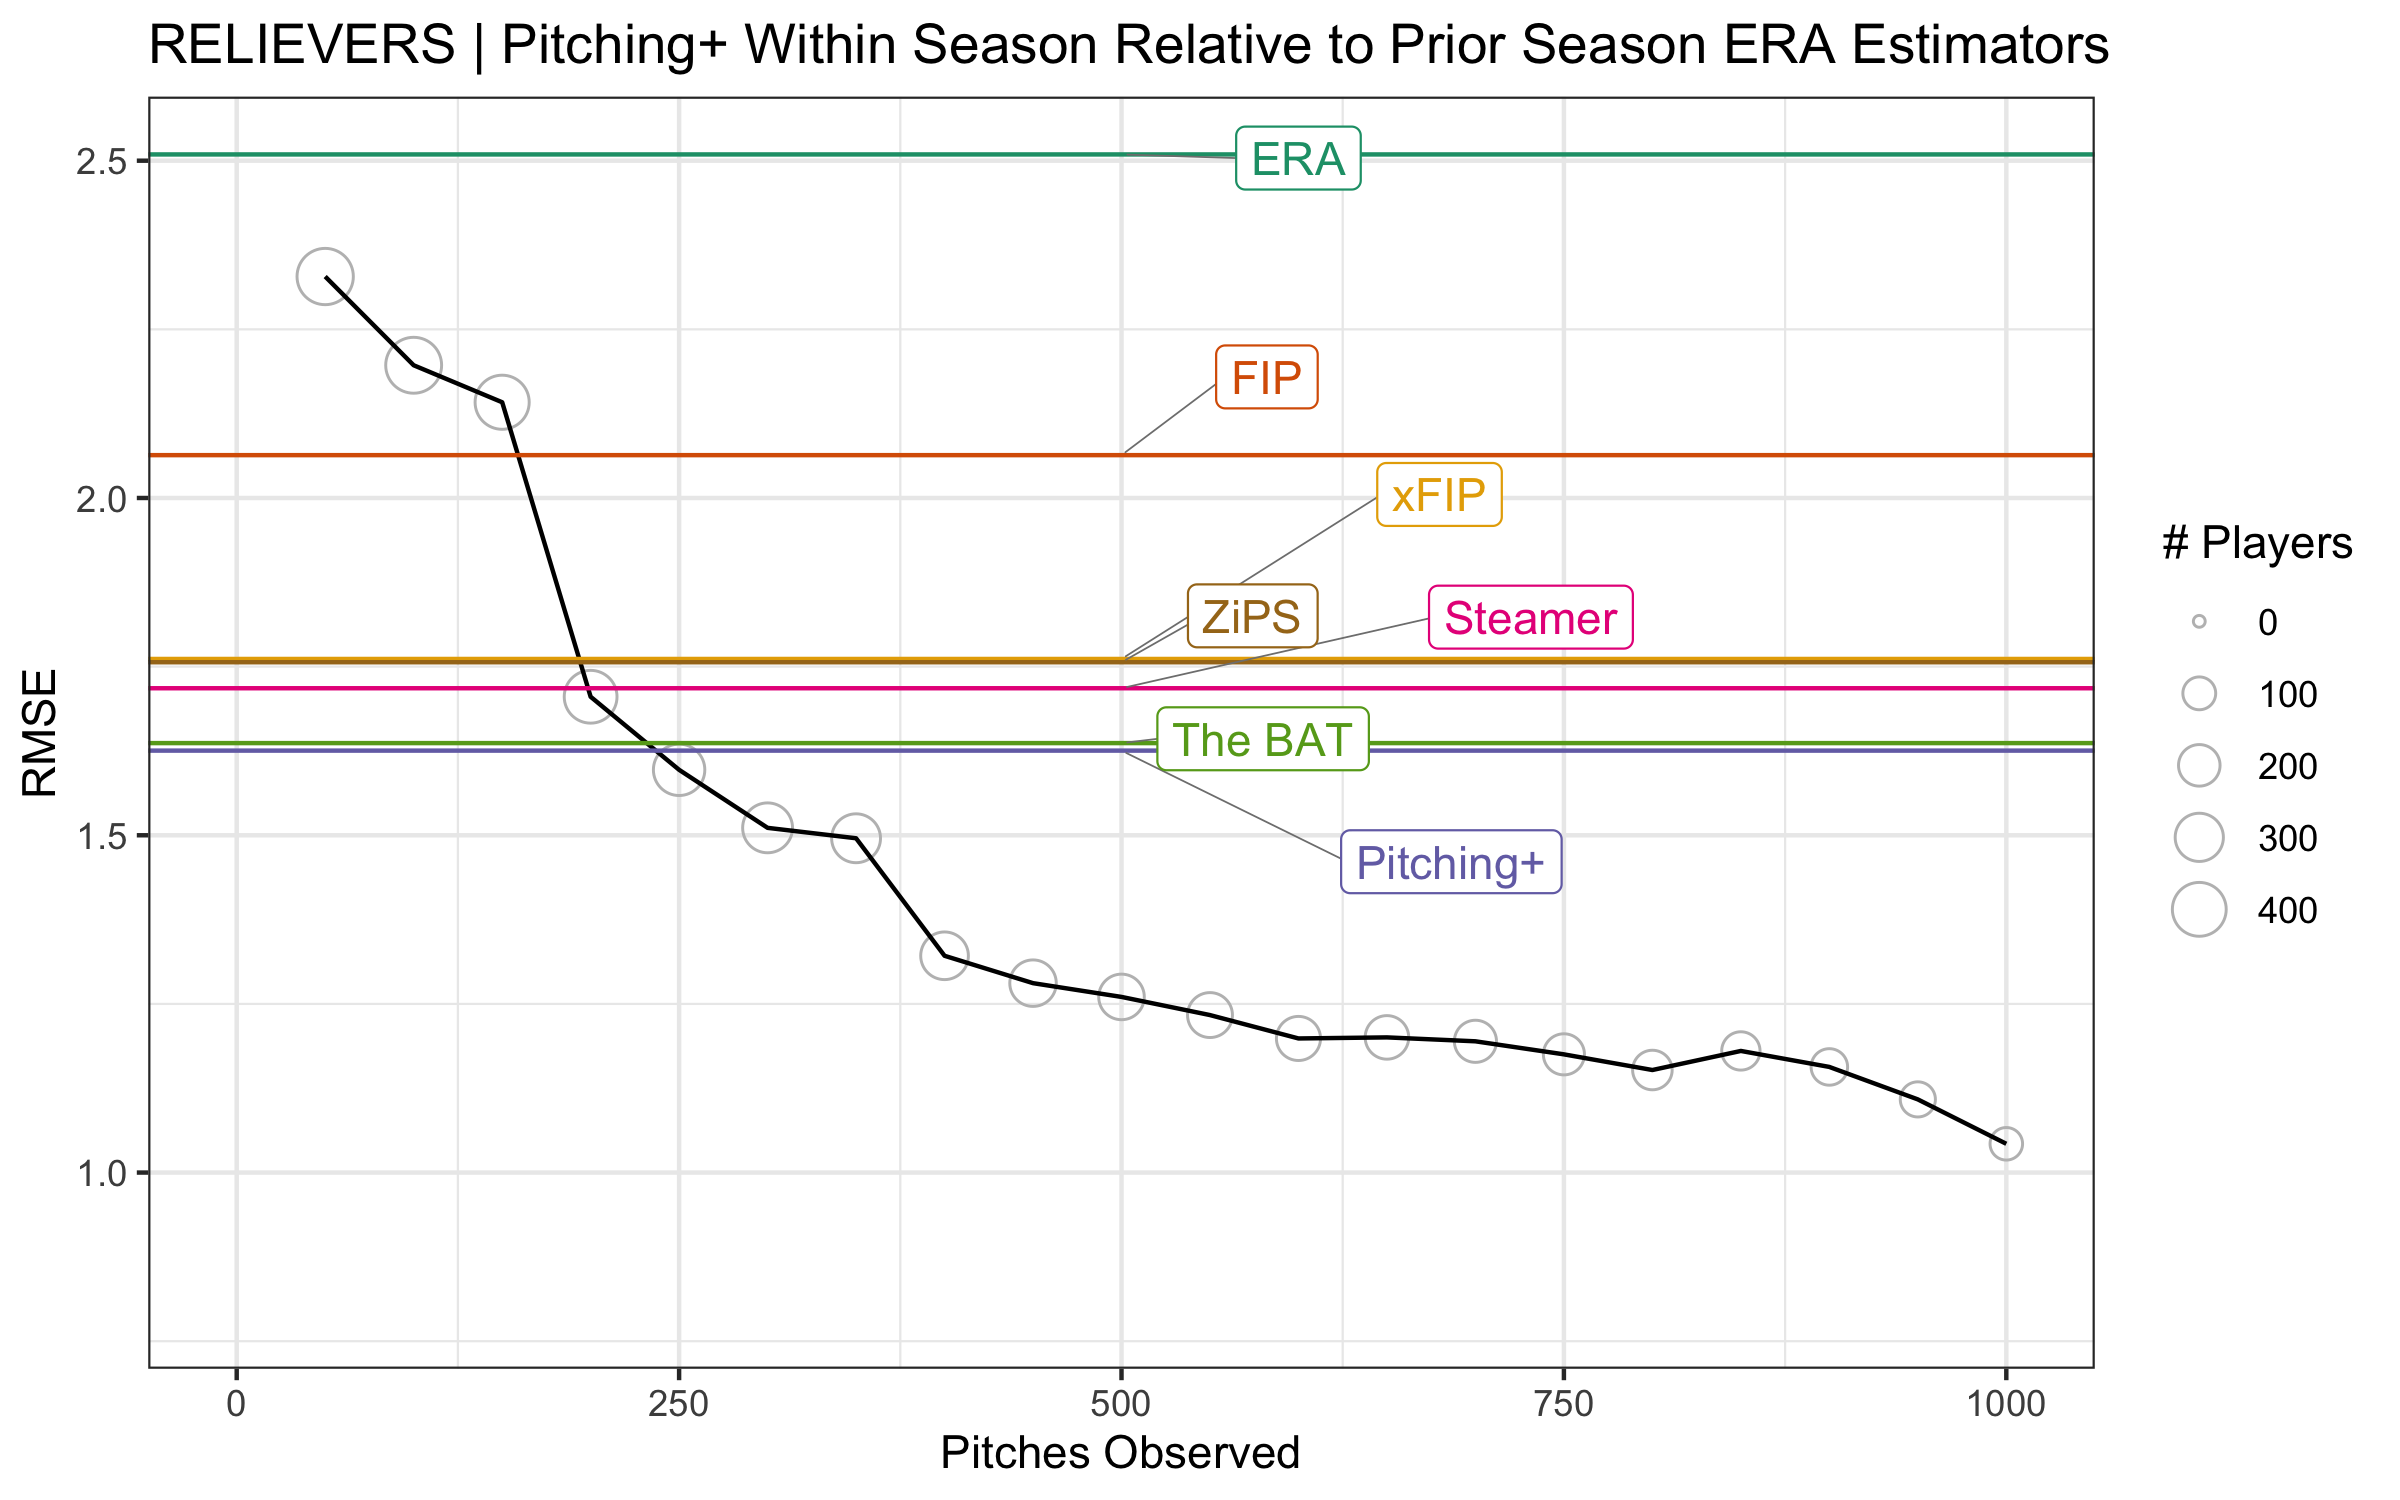
\includegraphics[width = \textwidth]{images/pitching_plus.png}\\
    \color{ricegray} \footnotesize https://library.fangraphs.com/pitching/stuff-location-and-pitching-primer/
  \end{frame}

  \begin{frame}{The Conundrum}
    \begin{columns}
      \begin{column}{0.5\textwidth}
        \centering
        Variable Importance\\
        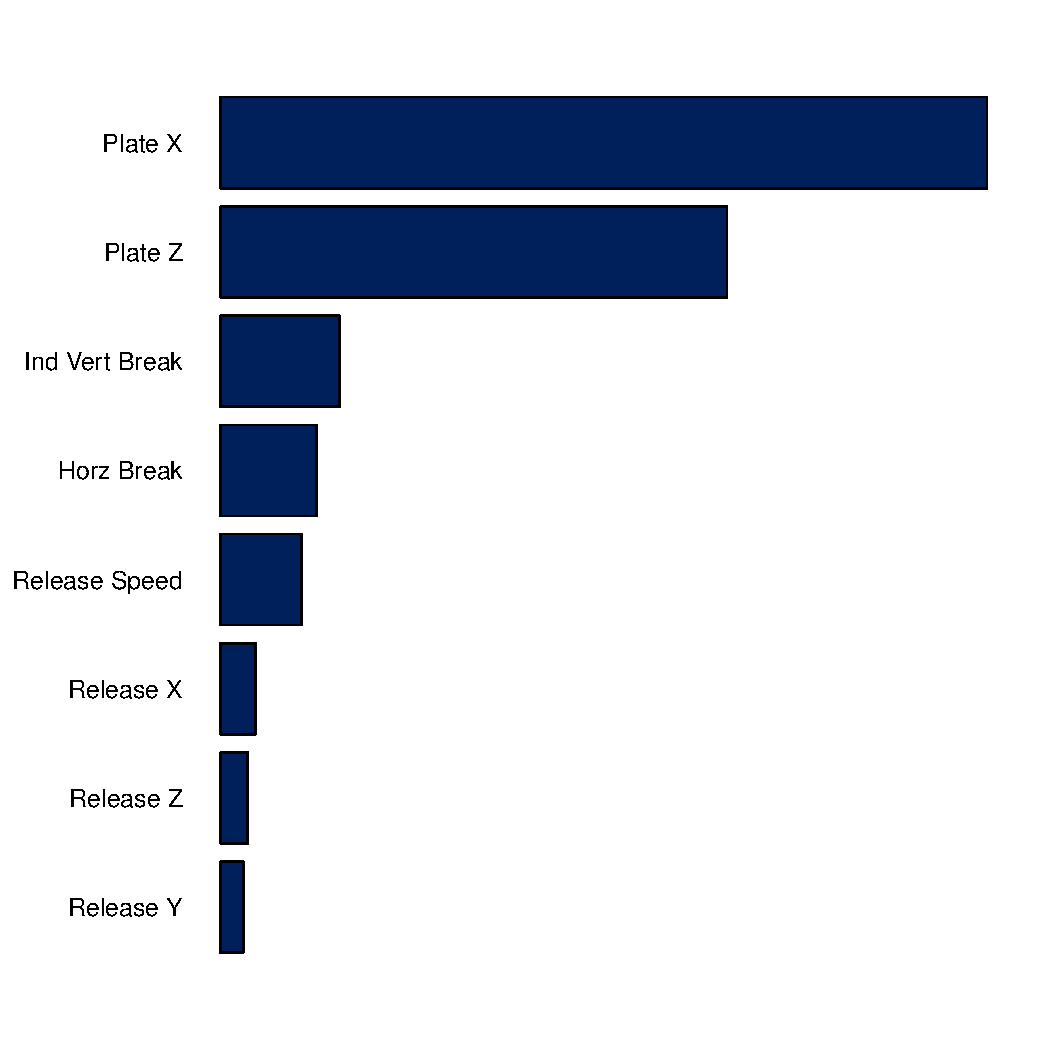
\includegraphics[width = \textwidth]{images/feature_importance.pdf}
      \end{column}
      \begin{column}{0.5\textwidth}
        \centering
        Variable Reliability*\\
        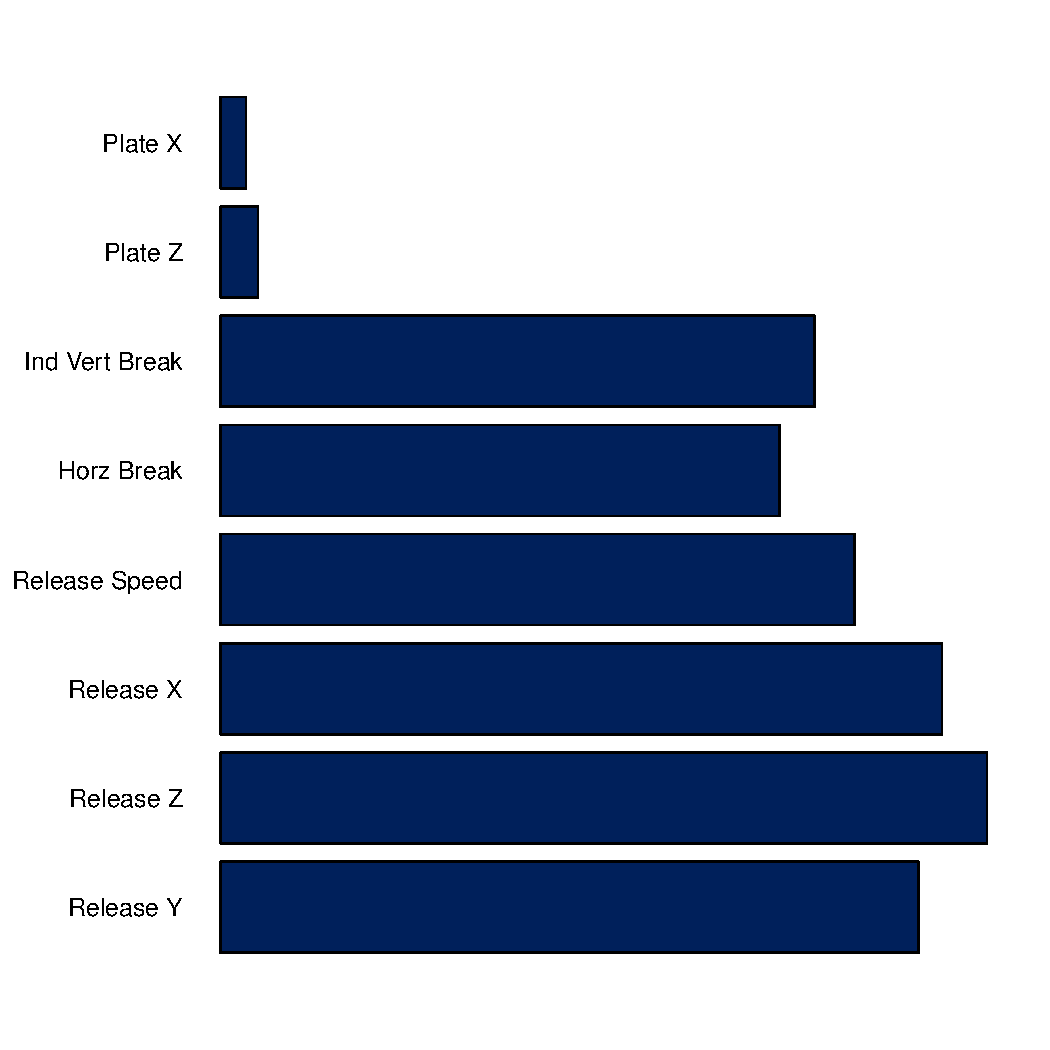
\includegraphics[width = \textwidth]{images/feature_reliability.pdf}
      \end{column}
    \end{columns}
    \scriptsize \color{ricegray}
    \vfill
    * (between-pitcher variance) / (total variance); varies by pitch type (RHB FB here)
  \end{frame}

  \begin{frame}{An Example}
    \begin{columns}
      \begin{column}{0.2\textwidth}
        \centering
        Pitch A\\
        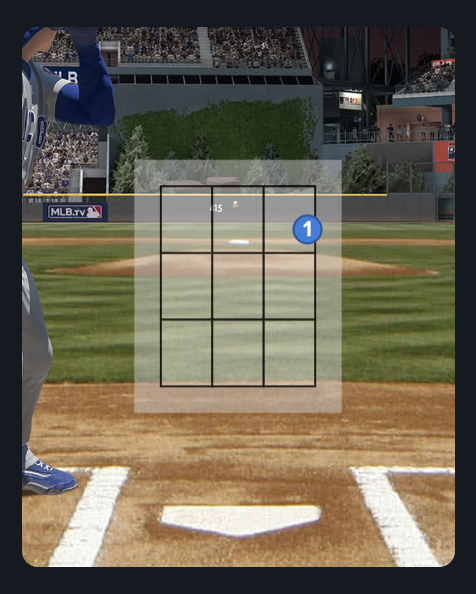
\includegraphics[width = \textwidth]{images/pitch_on_edge}
      \end{column}
      \begin{column}{0.8\textwidth}
        \begin{itemize}
          \item 91 mph FB
          \item 15 inches rise
          \item located on the edge of the zone
          \item 68\% called strike, 11\% foul, 8\% ball in play,\\
            8\% called ball, 5\% swinging strike ($-0.04$ runs)
        \end{itemize}
      \end{column}
    \end{columns}
    ~\\
    ~\\
    \begin{columns}
      \begin{column}{0.2\textwidth}
        \centering
        Pitch B\\
        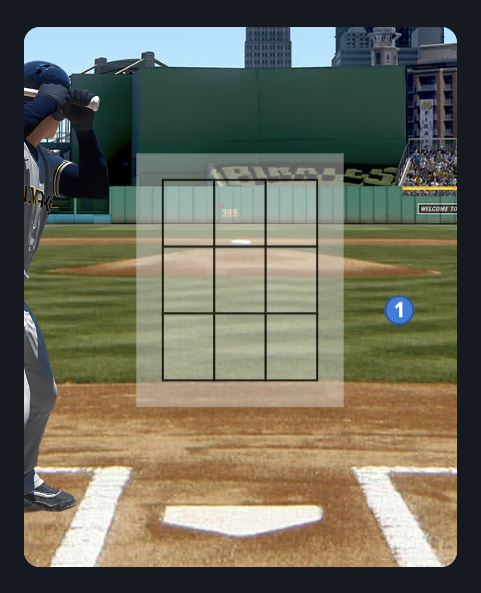
\includegraphics[width = \textwidth]{images/pitch_outside}
      \end{column}
      \begin{column}{0.8\textwidth}
        \begin{itemize}
          \item 98 mph FB
          \item 20 inches rise
          \item located a foot off of the plate
          \item 99.6\% called ball ($+0.04$ runs)
        \end{itemize}
      \end{column}
    \end{columns}
  \end{frame}

  \begin{frame}{Two Sources of Noise}
    \begin{enumerate}
      \item Random variation in the outcome given the pitch trajectory
      \begin{itemize}
        \item This is addressed by Pitching+, PitchingBot, etc.
      \end{itemize}
      ~\\
      \item Random variation in the pitch trajectory itself
      \begin{itemize}
        \item This is NOT addressed by Pitching+, PitchingBot, etc.
      \end{itemize}
    \end{enumerate}
  \end{frame}

  \begin{frame}{The Approach}
    \begin{enumerate}
      \item Fit a model to predict pitch outcome given its trajectory
      \begin{itemize}
        \item We use gradient boosting, not the focus today
      \end{itemize}
      ~\\
      \item Estimate the probability distribution over pitch trajectories
      \begin{itemize}
        \item Depends on pitcher, batter side, count, etc.
      \end{itemize}
      ~\\
      \item Apply the model {\color{riceblue} 1.} to the distribution {\color{riceblue} 2.}
      \begin{itemize}
        \item As opposed to applying the model to the observed pitches
      \end{itemize}
    \end{enumerate}
  \end{frame}

  \begin{frame}{Bayesian Hierarchical Model}
    \begin{itemize}
      \item We model each pitch as multivariate normal in 9 dimensions
      \begin{itemize}
        \item x/y/z release point, x/y/z release velocity, x/y/z acceleration
      \end{itemize}
      \item Mean $\mu \in \mathbb{R}^9$ includes additive effects for pitcher, count, batter side and strike zone height
      \item Covariance $\Sigma \in \mathbb{R}^{9 \times 9}$:
      \begin{itemize}
        \item Diagonal elements (variance) include multiplicative effects for pitcher, count
        \item Off-diagonal elements (correlation) vary by pitcher
      \end{itemize}
      \item We find the maximum {\it a posteriori} (MAP) model fit using the \texttt{optimize} function (automatic differentiation) from cmdstanr
    \end{itemize}
  \end{frame}

  \begin{frame}{Dylan Cease's Slider vs RHB in 0-0 Counts}
    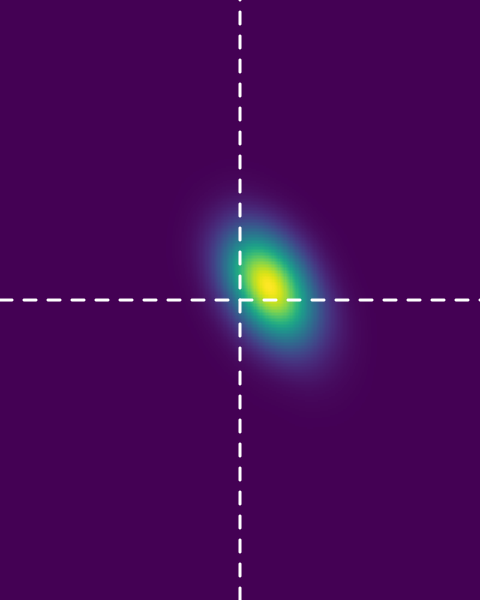
\includegraphics[width = 0.45\textwidth]{images/656302_SL_R_0_0_break.png}
    \hfill
    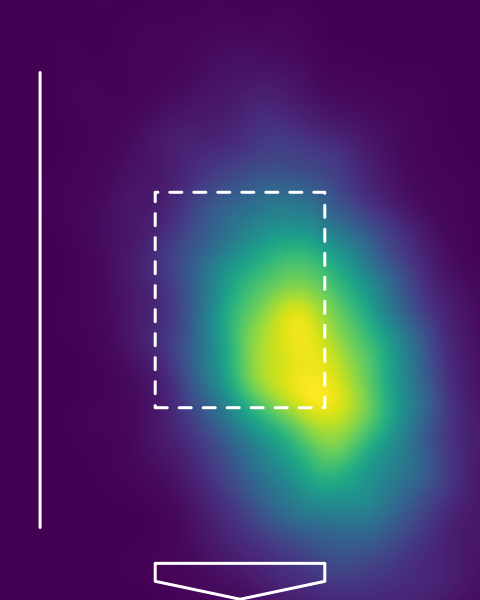
\includegraphics[width = 0.45\textwidth]{images/656302_SL_R_0_0_plate.png}
  \end{frame}

  \begin{frame}{Dylan Cease's Slider vs RHB in All Counts}
    \vfill
    \centering
    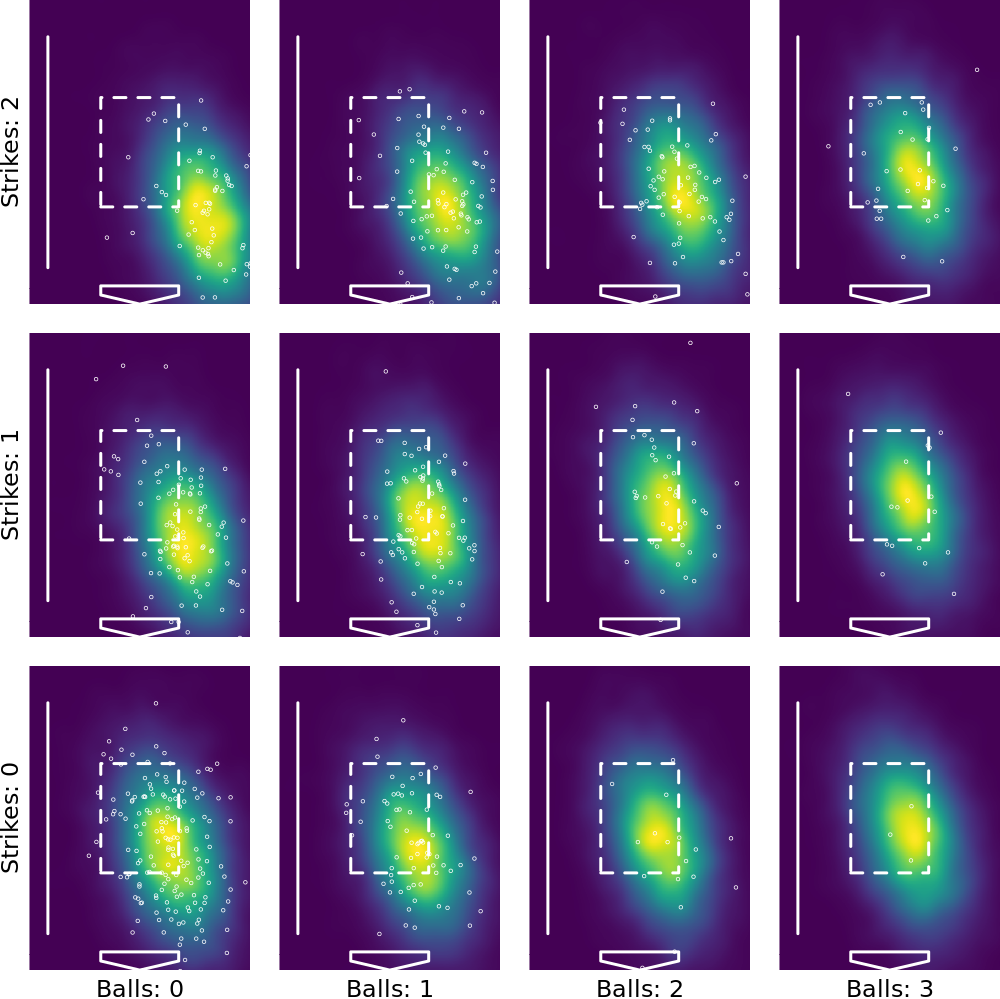
\includegraphics[height = 0.85\textheight]{images/656302_SL_R_plate.png}
  \end{frame}

  \begin{frame}{Does It Work?}
  \end{frame}

  \begin{frame}{More to Come!}
  \end{frame}

  \begin{frame}{Where to Find Us}

    {\color{ricegray} github.com/}{\color{ricerichblue}saberpowers/predictive-pitch-score}\\
    ~\\
    {\color{ricegray} linkedin.com/in/}{\color{ricerichblue}saberpowers}\\
    {\color{ricegray} twitter.com/}{\color{ricerichblue}saberpowers}\\
    ~\\
    {\color{ricegray} twitter.com/}{\color{ricerichblue}fiftycente1}
  \end{frame}

\end{document}
